\documentclass[12pt,letterpaper,english,bibliography=totocnumbered, abstract=on]{scrartcl}

\usepackage{indentfirst}
\usepackage[titletoc]{appendix}
%\usepackage{fullpage}
%\usepackage{subfiles}
\usepackage[T1]{fontenc}
\usepackage[latin9]{inputenc}
\usepackage{color}
\usepackage{babel}
\usepackage{verbatim}
\usepackage[unicode=true,pdfusetitle,
bookmarks=true,bookmarksnumbered=false,bookmarksopen=false,
breaklinks=true,pdfborder={0 0 0},pdfborderstyle={},backref=false,colorlinks=true]
{hyperref}
\hypersetup{linkcolor=blue,citecolor=blue,urlcolor=blue}

\usepackage{booktabs}
\usepackage{multirow}
\usepackage{adjustbox}
\usepackage{threeparttable}
\usepackage[table]{xcolor}
\usepackage{csquotes}
\usepackage{soul} % for hiliting text: \hl

\usepackage[backend=biber, style=authoryear, maxbibnames=99, dashed=false]{biblatex}
\setlength\bibitemsep{2\itemsep}
%\addbibresource{mylibrary.bib}
\addbibresource{../CRB.bib}

\usepackage{pdfpages}
\usepackage{float} % Allows use of H to place floats

\usepackage{pgfgantt}

\usepackage{framed}
\usepackage{amsmath}

% Prevent page breaks within paragraphs
% https://tex.stackexchange.com/questions/21983/how-to-avoid-page-breaks-inside-paragraphs
\widowpenalties 1 10000

% add verticle space after a paragraph
\setlength{\parskip}{1em}

\begin{document}

\title{Parameters for Coconut Rhinoceros Beetle Modeling}

\author{Aubrey Moore}

\maketitle
%\footnote{\url{https://github.com/aubreymoore/2020-FS-CRB-biocontrol-project/blob/master/combined-proposal.pdf}}
\newpage
\tableofcontents
\pagebreak

\begin{abstract}
	This document represents an attempt to extract parameters for modeling coconut rhinoceros beetle (CRB) population dynamics from the literature. A couple of review articles provided a good starting point: \cite{bedford_biology_1980} and \cite{pallipparambil_new_2015}. The only published journal article on modeling CRB population dynamics, \cite{hochberg_model_1991}, was also a useful reference. 
\end{abstract}

\section{Population structure}

\subsection{Table from \cite{abidin_population_2014}}
\begin{center}
	\includegraphics[width=0.7\linewidth]{../images/abidin2014}
\end{center}

Proportion of adults in zero burning is 2.9\%, in partial burning it is 3.2\%.

\subsection{Table from \cite{gressitt_coconut_1953}}
\begin{center}
	\includegraphics[width=0.7\linewidth]{../images/gressitt1953}
\end{center}

\begin{itemize}
	\item Proportion of population in adult stage: 16.0\%
	\item Proportion of adults in live coconut palms: 73.5\%
	\item Proportion of population in live coconut palms: 11.8\%
\end{itemize}

\section{Coconut rhinoceros beetle (CRB) biology}

Note: This section was written in preparation for an article on using harmonic radar to detect CRB breeding sites.

\subsection{Life cycle and feeding behavior}

\textit{Oryctes rhinoceros} (Linnaeus 1758) (Coleoptera: Scarabaeidae: Dynastinae), commonly known as the coconut rhinoceros beetle (CRB) is a major pest of  coconut and oil palm. CRB undergo complete metamorphosis with four distinct life stages: egg, larva, pupa and adult. Larvae feed exclusively on dead and decaying vegetation and cause no economic damage. Damage is done by adults of both sexes which bore into palm crownshafts to feed on sap to fuel their flight muscles. This boring activity typically damages several fronds developing within the crownshaft. When these fronds emerge and expand several weeks afterwards, the damage becomes visible as v-shaped cuts, a distinctive sign of CRB damage. Palms are killed only when the apical meristem (growing tip), located at the base of the crownshaft, is damaged by CRB boring activity. However, mortality caused by CRB is rare unless CRB population densities are high and palms are attacked simultaneously by multiple adults. Adults reside in palms only briefly, exiting bore holes within a few days to aggregate at breeding sites where they mate and lay eggs. Each CRB may feed up to 6 times during its adult lifetime \parencite{vander_meer_indirect_1975}, boring a new hole each time.

From a survey of Ngiwal Village in the Palau Islands \cite{gressitt_coconut_1953} estimated that 88\% of the CRB population occurred in breeding site aggregations. The remaining 12\% were adults which briefly left breeding sites to feed on sap in palm crowns. Breeding sites are found in a wide variety of decaying plant material including dead standing coconut palms, fallen coconut logs, rotting coconut stumps, and decaying wood of many tree species, piles of compost, sawdust, and manure. Severe CRB outbreaks often occur in response to massive amounts of decaying vegetation gemerated by typhoons, large scale land clearing and wars.

\subsection{Invasion history}

CRB is endemic to the tropical Asia region (including South East Asia).
The beetle was inadvertently introduced into the Pacific in 1909 when infested rubber tree plants were transported to Samoa from Sri Lanka (previously known as Ceylon). The pest rapidly multiplied in Samoa and subsequently spread to several nearby Polynesian islands. Separate invasions further distributed CRB through Palau, parts of Papua New Guinea, and other Pacific nations through disruptions and uncontrolled movements during World War II . The invasive phase of the beetle was brought under control by the discovery and distribution of a viral biocontrol agent, Oryctes rhinoceros nudivirus (OrNV). OrNV causes persistent population suppression on many of the CRB infested Pacific Islands where it was introduced.

Detection of CRB on Guam in 2007 heralded a second wave of Pacific island invasions by this pest. Following a failed eradication attempt it was discovered that the Guam beetles are an OrNV resistant form which is being referred to as the CRB-G biotype . This problematic biotype has already spread to previously uninfested Pacific islands where it is damaging and killing coconut and oil palms.

\subsection{Eradication programs}

The recipe for eradicating coconut rhinoceros beetle from an island is simple:

\begin{itemize}
	\item find and destroy all active and potential breeding sites
	\item prevent re-infestation by closing invasion pathways
\end{itemize}

However, eradication of CRB from an island has proven extremely difficult once this pest has become established. There have been many CRB eradication attempts and some are currently in progress. But there has been only one success. This was accomplished on the tiny (36 km\textsuperscript{2}) Niuatoputapu Island (also known as Keppel Island), which lies between Samoa and Tonga \parencite{catley_coconut_1969}. During a period spanning 1922 to 1930 all CRB breeding sites were located and destroyed.

We suggest that harmonic radar may be useful for efficient detection of CRB breeding sites, thus improving probability of successful eradication.

\section{Parameters used in the Hochberg and Waage model}

Table from \cite{hochberg_model_1991}:
\begin{center}
	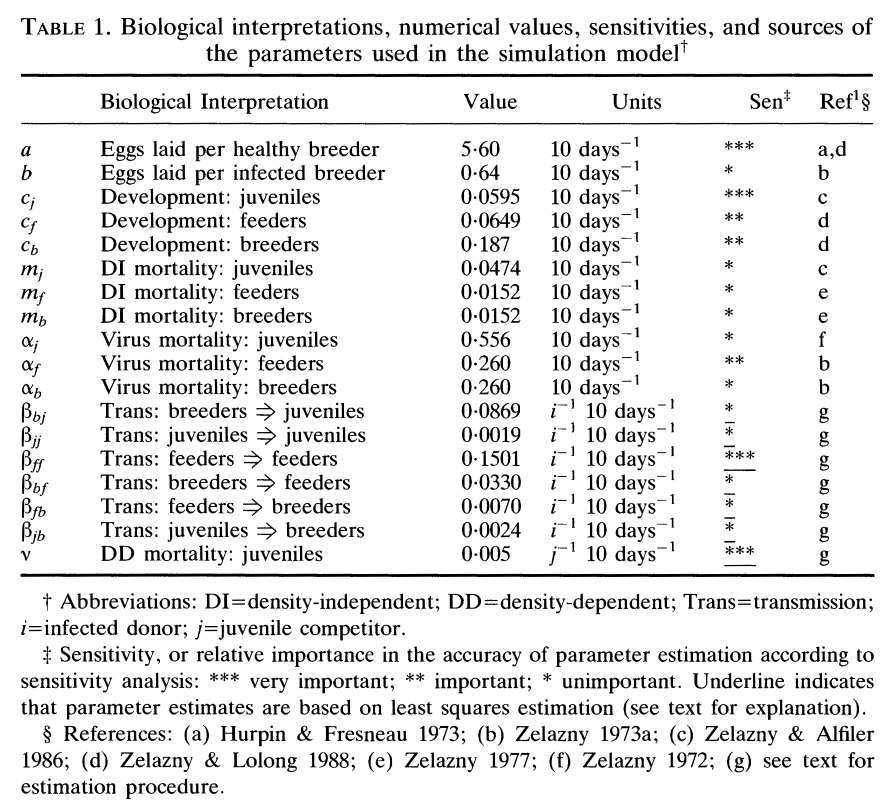
\includegraphics[width=0.7\linewidth]{../images/hochberg-model-params}
\end{center}


\section{Life cycle}

Table from \cite{bedford_biology_1980}. Note that the column for CRB, \textit{Oryctes rhinoceros}, was compiled using data from 4 sources:

\begin{center}
	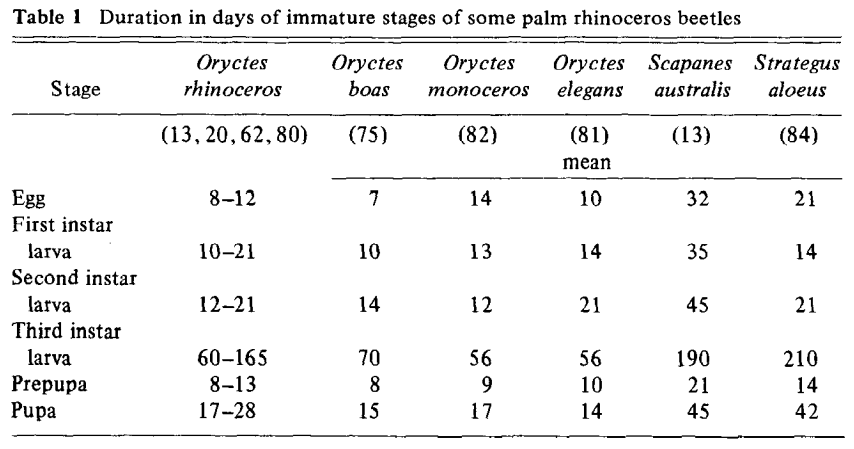
\includegraphics[width=0.7\linewidth]{../crb-life-cycle}
\end{center}

\section{Life table data}

"A lab study by Indiravathi (2001) reported that approximately 63\% of eggs and 87\% of larvae successfully developed into adults." [\cite{pallipparambil_new_2015}]

"Small improvements in the average survival of
larvae would explain the post-typhoon increases in
Rhinoceros Beetle populations so often observed on
Pacific islands. Assuming survival from oviposition
to adult emergence is near 2 percent in a stable pop-
ulation: a posttyphoon generation might increase
2.5 times with an average 5 percent survival in
the numerous palm logs felled by the storm. A
population decline would be expected only when
preadult mortality exceeds 98 percent." [\cite{hinckley_ecology_1973}]

\section{Life span and generation time}

"The total life span in Palau may range from 150 to about 270 days, and I assume the average under normal conditions to be about 200 days. The pre-incubation period is about 12 to 20 days. The period from the of an egg to first egg of the next generation may be as little as 115 days. Thus, given favorable conditions, more than 3 generations my develop in one year." [\cite{gressitt_coconut_1953}]

"Unfavorable environmental conditions reduces larval size and prolongs
development up to 420 d (Catley, 1969)." [\cite{pallipparambil_new_2015}]

\section{Larval food conversion}

"The minimum volumes per grub were 400 cc in a coconut log; 5000 cc in a kapok log; 7000 cc in a breadfruit log; 7000 cc in sawdust; and 9000 cc in grass compost." [\cite{hinckley_ecology_1973}]
\section{Fecundity}

"A female lays 70 to more than 100 eggs in its lifetime. Taking 90 as the average number of eggs laid by one female and assuming the sex ratio to be one female to one male, with an average life-cycle of 4 months to middle of egg-layng period for each female), the theoretical figure of 186,390 progeny per original female during one year (16,995,293,890 by the end of two years) is obtained." [\cite{gressitt_coconut_1953}]

"Both sexes mate several times and from studies of spermatophore residues in the bursa copulatrix
of field collected females Hoyt (undated) estimated that there is a maximum of eight matings. However,
field collected females have produced fertile eggs up to 130 days after being confined singly in cans of
rotting sawdust which suggests that multiple matings are not essential. Egg production varies considerably
depending on the longevity of the beetle and the suitability of the oviposition medium. Menon and Pandalai (1958) recorded up to 152 eggs per female although 90 - 100 would be more usual." [\cite{catley_coconut_1969}]

\section{Sex ratio}

"Of 282 specimens examined from Palau and Samoa, 142 were males and 140 were females. This suggests a ratio of 1.014 males to one female." [\cite{gressitt_coconut_1953}]

\section{Flight distances}
"The beetle is thought to prefer short flights, but
is capable of long flights if local conditions are unfavorable (Catley, 1969). A
lab study demonstrated that palm-fed tethered adult beetles had a flight
potential of 2-3 h, covering the equivalent of 2-4 km (Hinckley, 1973).
Reports of long distance flight by \textit{O. rhinoceros} include adults flying toward
light on a ship anchored 700 m from shore (Catley, 1969), marked adults
recaptured at 900 m within 3d and approximately 1600 m within a month
(Cumber, 1957). Kamarudin and Wahid (2004) used mark-release-recapture
studies to determine the flight range of \textit{O. rhinoceros} in oil palm replanting
regions in Malaysia; their results suggested that the adults moved at the rate of
10-23 m/day and up to 1.3 km/week." [\cite{pallipparambil_new_2015}]

\section{Number of adult feeding events (=attacks)}

\cite{vander_meer_per_1987} indicates that adult CRB feed 6 times between days 30 and 150 after eclosion from the pupa (see figure 4 in the article).

\newpage
\section{Probability of a palm dying as the result of CRB attacks}

$$
p(Mortality)=
\begin{cases}
0, & \text{if $AR < LAR0$} \\
\frac{AR-LAR0}{LAR1-LAR0}, & \text{if $LAR0 <= AR <= LAR1$} \\
1, & \text{if $AR > LAR1$}
\end{cases}
$$

Where:

$p(Mortality)$ is the probablility of mortality of a palm tree immediately following a CRB attack
	
$AR$ is the attack rate which is the number of simultaneous attacks (=bore holes) during a time period. In this model the time period is one CRB generation.

$LAR0$ is the highest attack rate which results in 0\% mortality as a result of CRB.

$LAR1$ is the lowest attack rate which results 100\% mortality as a result of CRB.

\begin{center}
	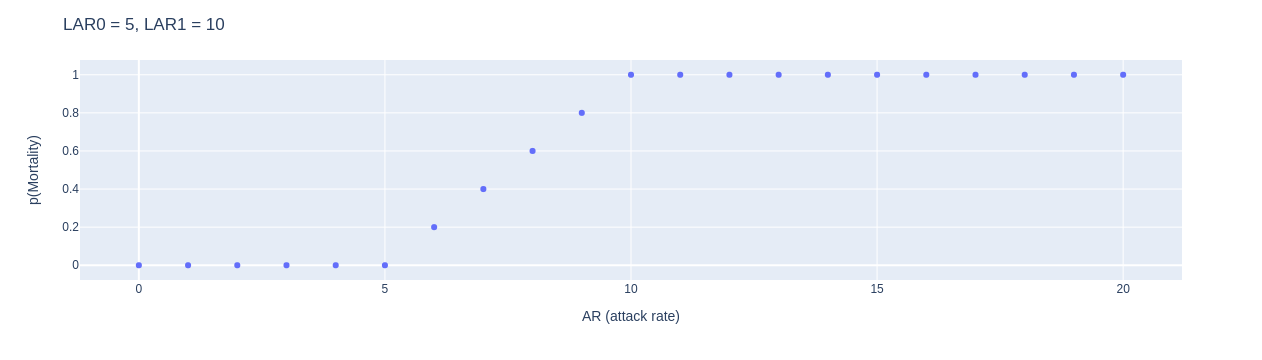
\includegraphics[width=\linewidth]{../images/pmort}
\end{center}


\section{Detection level for economic damage}

\cite{hinckley_ecology_1973}:

"The final goal should be a population reduction below the level at which economic damage\textsuperscript{3} can be detected (Hinckley 1966).

\textsuperscript{3}About 7.5 beetles/hectare (3/acre) on plantations in Western Samaoa."

\section{Density of coconut palms on Guam}

Estimated number of \textit{Cocos nucifera} with DBH > 5 inches growing on forested land on Guam (63,383 acres) is 1,162,494. [\cite{donnegon_guams_2004}] 

This is 18.21 coconut palms per acre (=	45.00 per ha).

\newpage
\printbibliography

\end{document}
